\maketitle
\section{SM and beyond: Allowed, forbidden and discovery process}

The feynman diagrams are showed below. Every process is allowed according
to conserved quantities, with the possible exception of number 5 where
there should be a muon neutrino, but because of neutrino oscilliation
it could be allowed depending on how long after the reaction the final
particles were measured.

\begin{itemize}
      	  \item Electromagnetic
      	    \begin{itemize}
      	      \item 1, 2, 3, 4, 6, 8, 11, 12, 13, 14, 15, 16, 20
      	    \end{itemize}
      	  \item Weak
      	    \begin{itemize}
      	      \item 3, 4, 5, 7, 8, 10, 11, 13, 15, 18, 19, 20
      	    \end{itemize}
	  \item Strong
	    \begin{itemize}
	      \item 1, 2, 4, 6, 8, 9, 12, 14, 16, 17
	    \end{itemize}
\end{itemize}
\newpage
There are four decays present, $\tau^+$, two $H$ and a $\Upsilon(3s)$.

$\tau^+ \rightarrow \mu^+\nu_e\bar{\nu}_{\tau}$\newline
Since the branching ratio for $\tau$ to $\mu$ is about the same as
with $\mu$ to $e$  and their mass difference is large we can use the relationship 
\begin{flalign}
  &\frac{1}{\tau_l} = G_f^2 m_l^5\\
  &\frac{\tau_{\tau}}{\tau_{\mu}} = \frac{m_{\mu}^5}{2m_{\tau}^5}\\
  &\text{the factor 2 comes from that $\tau$ has 2 leptonic decays}\\
  &\tau_{\tau} = \frac{\tau_{\mu}}{2}\left(\frac{m_{\mu}}{m_{\tau}}\right)^5%
  \approx 2.0\times 10^{-12}
\end{flalign}
For the branching ratio for three-body weak decay, Sargent rule states
\begin{flalign}
  &\frac{\Gamma_i/\Gamma}{\tau_{\tau}} = G_f^2m_{\tau}^5\\
  &\Gamma_i/\Gamma = \tau_{\tau}G_f^2m_{\tau}^5
\end{flalign}

$H \rightarrow gg,\, H \rightarrow Z\gamma$\newline
The lifetime of the higgs goes as $1/m_H^2$ which is of the order $10^{-22}$
As for the branching ratio it goes proportional as the vertex matrix element $\mathcal{M}$
\[ \frac{BR}{\tau_{H}} = \left(\frac{m_f}{V}\right)^2\]
where $V = (\sqrt{2}G_f)^{-1/2}$


\paragraph{Suppresion/forbidding}
In process 9, 11, 12 and 20 there are a large mass difference from initial to final, which
can cause supression of these processes.
\newpage
\paragraph{Importance:}
\paragraph{Process 3}
This process would show that supersymmetric particles exists and there be a breakthrough in 
particle physics.
\paragraph{Process 4 \& 8}
These are of interest because of our circular accelerators and these reactions are there plentiful
and much studied.
\paragraph{Process 10}
Quarks going into pure weak bosons shows the ability of the $W^{\pm}$ to change the quarks from
particle to anti particle and vice versa.
\paragraph{Process 11}

\paragraph{Process 14}
Both top and higgs production is of interest since they are our heavy weight champions and therefore
has limitd lifetime. The uniqeness of the tops ability to be single due to its short lifespan is a
golden oppurtunity to see quarks alone.
\paragraph{Process 18}
$J/\psi$ is a highly measured and has a narrow width, so it has been used as a calibartion particle
when setting up new detectors.
\newgeometry{left=0.5cm,right=0.5cm,top=0.2cm,bottom=1.3cm}
\begin{figure}[h]
  \centering
  \begin{subfigure}[b]{0.3\textwidth}
    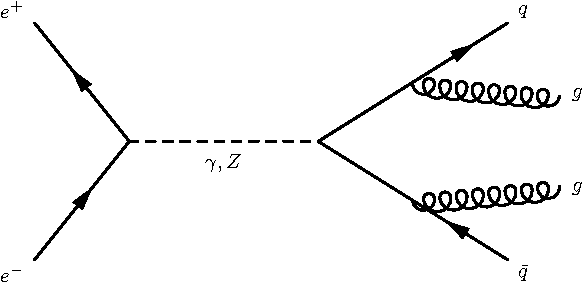
\includegraphics[width=\textwidth]{../dia/01.pdf}
    \caption{$e^+e^- \rightarrow q\bar{q}gg$}
    \label{fey:1}
  \end{subfigure}%
  ~
  \begin{subfigure}[b]{0.3\textwidth}
    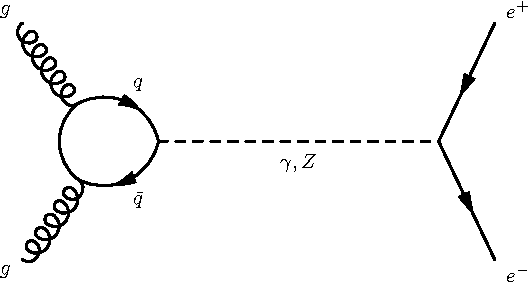
\includegraphics[width=\textwidth]{../dia/02.pdf}
    \caption{$gg\rightarrow e^+e^-$}
    \label{fey:2}
  \end{subfigure}%
  ~
  \begin{subfigure}[b]{0.3\textwidth}
    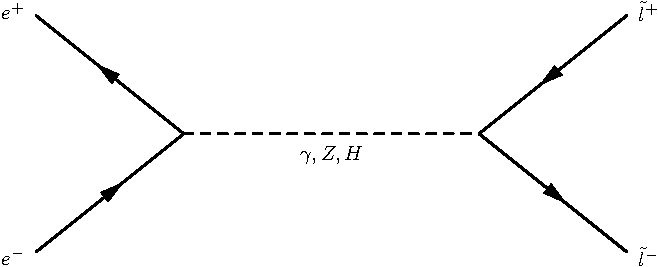
\includegraphics[width=\textwidth]{../dia/03.pdf}
    \caption{$e^+e^-\rightarrow \tilde{l}^+\tilde{l}^-$}
    \label{fey:3}
  \end{subfigure}
  \newline
  \newline
  \begin{subfigure}[b]{0.3\textwidth}
    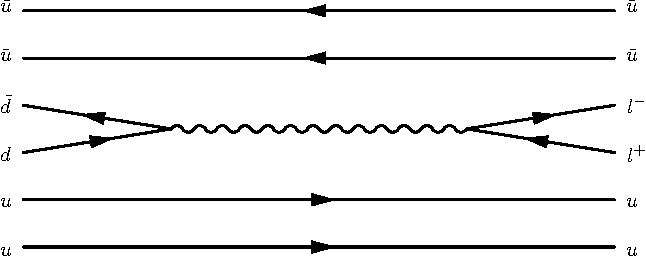
\includegraphics[width=\textwidth]{../dia/04.pdf}
    \caption{$p\bar{p}\rightarrow l^+l^-x$}
    \label{fey:4}
  \end{subfigure}%
  ~
  \begin{subfigure}[b]{0.3\textwidth}
    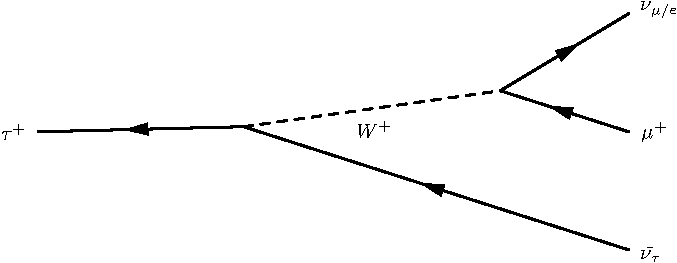
\includegraphics[width=\textwidth]{../dia/05.pdf}
    \caption{$\tau^+\rightarrow \mu^+\bar{\nu}_{\tau}\nu_{e/\mu}$}
    \label{fey:5}
  \end{subfigure}%
  ~
  \begin{subfigure}[b]{0.3\textwidth}
    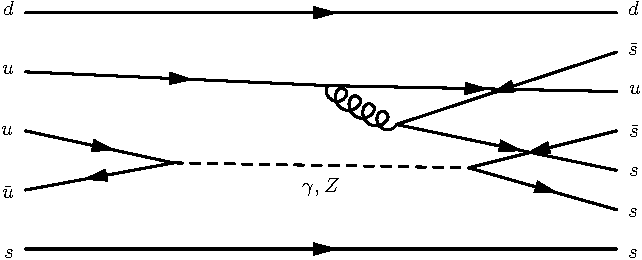
\includegraphics[width=\textwidth]{../dia/06.pdf}
    \caption{$k^-p\rightarrow \omega^-k^+k^0$}
    \label{fey:6}
  \end{subfigure}
  \newline
  \newline
  \begin{subfigure}[b]{0.3\textwidth}
    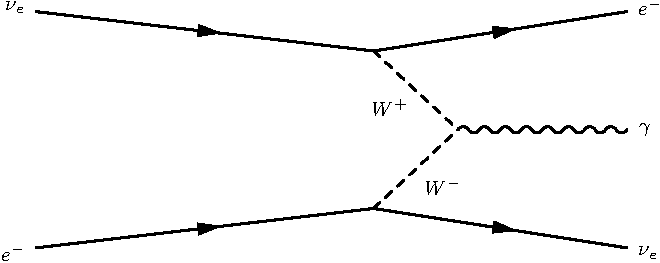
\includegraphics[width=\textwidth]{../dia/07.pdf}
    \caption{$e^-\nu_e\rightarrow \nu_e \gamma e^-$}
    \label{fey:7}
  \end{subfigure}%
  ~
  \begin{subfigure}[b]{0.3\textwidth}
    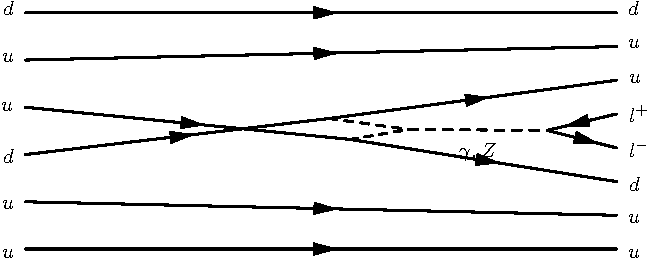
\includegraphics[width=\textwidth]{../dia/08.pdf}
    \caption{$pp\rightarrow ppl^+l^-$}
    \label{fey:8}
  \end{subfigure}%
  ~
  \begin{subfigure}[b]{0.3\textwidth}
    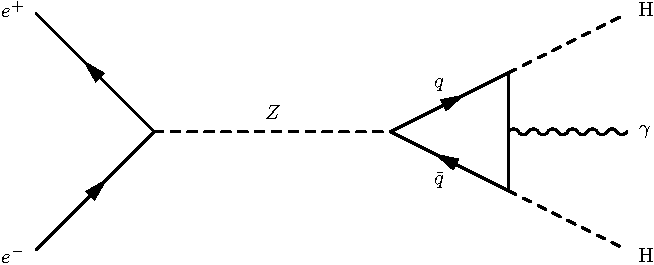
\includegraphics[width=\textwidth]{../dia/09.pdf}
    \caption{$e^-e^+ \rightarrow \gamma HH$}
    \label{fey:9}
  \end{subfigure}
  \newline
  \newline
  \begin{subfigure}[b]{0.3\textwidth}
    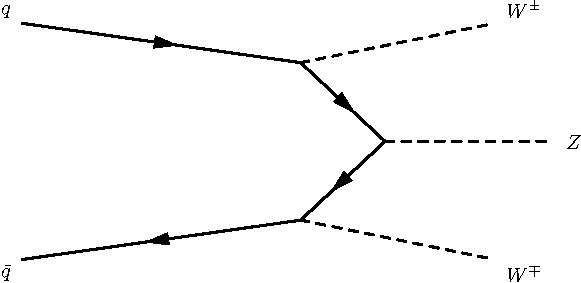
\includegraphics[width=\textwidth]{../dia/10.pdf}
    \caption{$qq\rightarrow W^{\pm}W^{\mp}Z$}
    \label{fey:10}
  \end{subfigure}%
  ~
  \begin{subfigure}[b]{0.3\textwidth}
    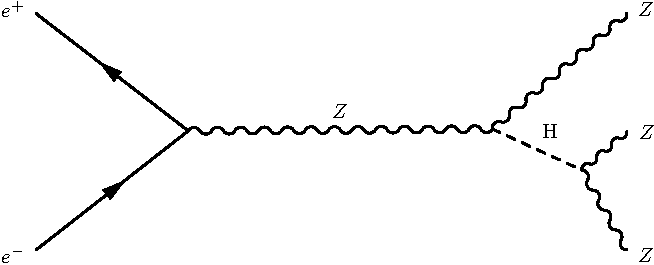
\includegraphics[width=\textwidth]{../dia/11.pdf}
    \caption{$e^-e^+\rightarrow ZZ$}
    \label{fey:11}
  \end{subfigure}%
  ~
  \begin{subfigure}[b]{0.3\textwidth}
    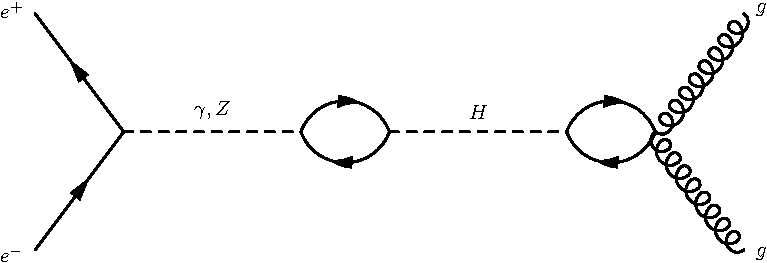
\includegraphics[width=\textwidth]{../dia/12.pdf}
    \caption{$e^-e^+\rightarrow H \rightarrow gg$}
    \label{fey:12}
  \end{subfigure}
  \newline
  \newline
  \begin{subfigure}[b]{0.3\textwidth}
    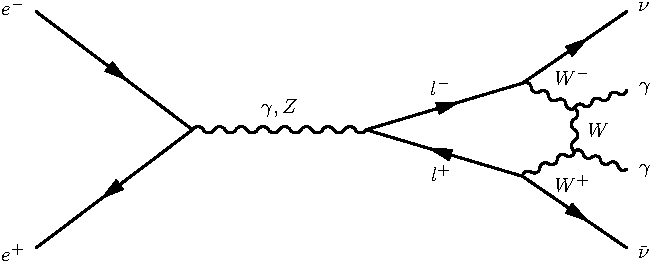
\includegraphics[width=\textwidth]{../dia/13.pdf}
    \caption{$e^+e^- \rightarrow \nu\bar{\nu}\gamma\gamma$}
    \label{fey:13}
  \end{subfigure}%
  ~
  \begin{subfigure}[b]{0.3\textwidth}
    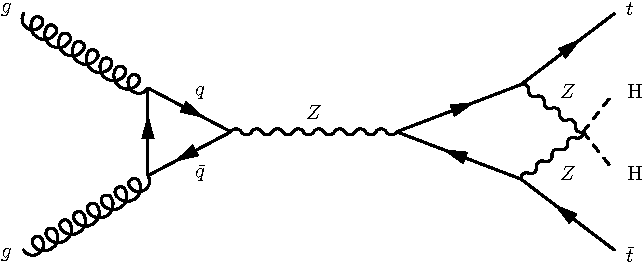
\includegraphics[width=\textwidth]{../dia/14.pdf}
    \caption{$gg\rightarrow t\bar{t}HH$}
    \label{fey:14}
  \end{subfigure}%
  ~
  \begin{subfigure}[b]{0.3\textwidth}
    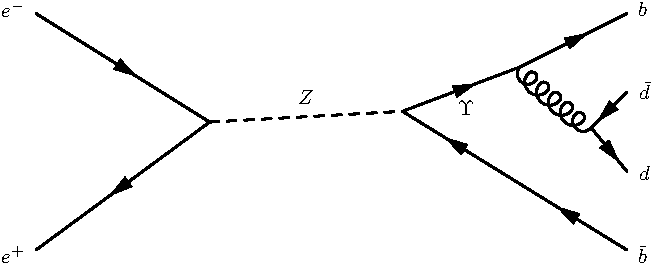
\includegraphics[width=\textwidth]{../dia/15.pdf}
    \caption{$e^+e^-\rightarrow \Upsilon(3s)\rightarrow B^0\bar{B^0}$}
    \label{fey:15}
  \end{subfigure}
  \newline
  \newline
  \begin{subfigure}[b]{0.3\textwidth}
    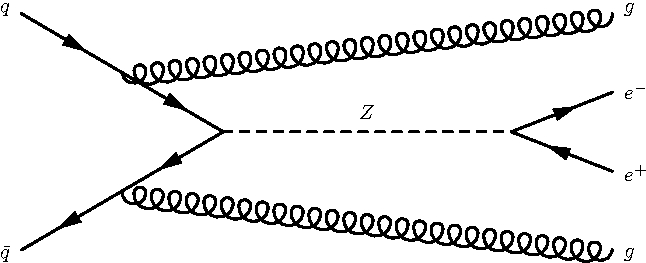
\includegraphics[width=\textwidth]{../dia/16.pdf}
    \caption{$q\bar{q}\rightarrow gge^-e^+$}
    \label{fey:16}
  \end{subfigure}
  ~
  \begin{subfigure}[b]{0.3\textwidth}
    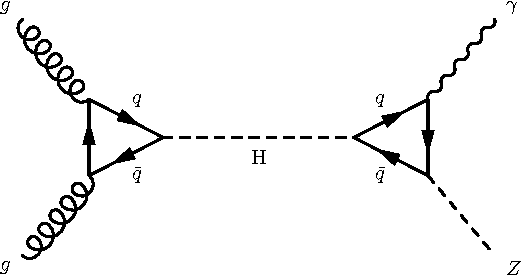
\includegraphics[width=\textwidth]{../dia/17.pdf}
    \caption{$gg \rightarrow Z\gamma$}
    \label{fey:17}
  \end{subfigure}%
  ~
  \begin{subfigure}[b]{0.3\textwidth}
    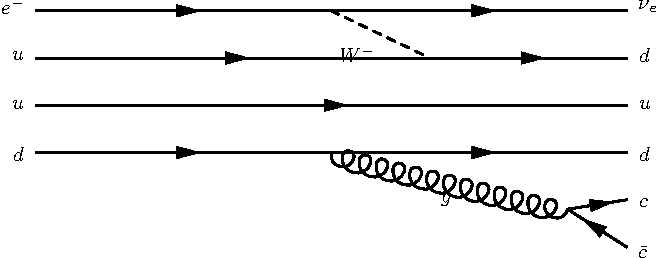
\includegraphics[width=\textwidth]{../dia/18.pdf}
    \caption{$gg\rightarrow t\bar{t}HH$}
    \label{fey:18}
  \end{subfigure}%
\end{figure}
\restoregeometry
\begin{figure}[h]
  \centering
  \begin{subfigure}[b]{0.3\textwidth}
    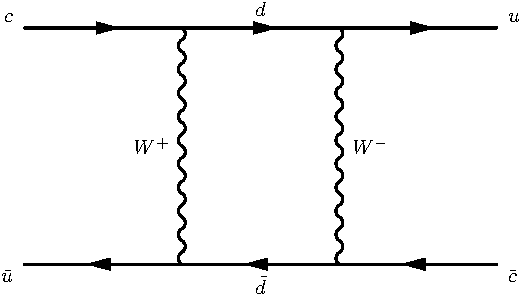
\includegraphics[width=\textwidth]{../dia/19.pdf}
    \caption{$D^0\longleftrightarrow \bar{D}^0$}
    \label{fey:19}
  \end{subfigure}
  ~
  \begin{subfigure}[b]{0.3\textwidth}
    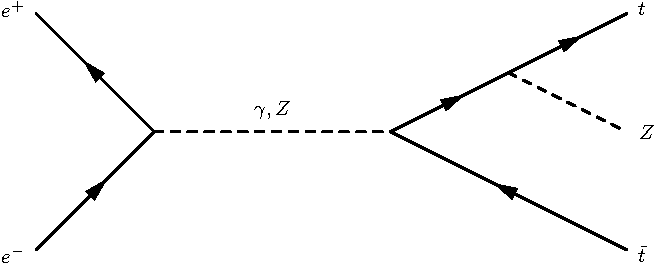
\includegraphics[width=\textwidth]{../dia/20.pdf}
    \caption{$e^+e^- \rightarrow t\bar{t}Z$}
    \label{fey:20}
  \end{subfigure}
\end{figure}
